\chapter{Análise dos Dados}\label{analise-dos-dados}

A análise dos dados será feita a partir dos dados coletados pelos testes realizados usando a ferramenta ApacheBench nas máquinas virtuais, cada uma utilizando um servidor HTTP diferente.\\
Os dados coletados nos testes foram tabelados e, para uma melhor análise, foram gerados gráficos dos mesmos.

\section{Algumas considerações}
Com a grande quantidade de dados coletados, 75 para cada servidor HTTP totalizando 150 testes, cada teste gerando 8 parâmetros, gerando 1.200 dados, os dados serão agrupados de acordo com a quantidade total de requisições feitas no teste. \\
Os gráficos serão divididos em 3 faixas de valores para a quantidade total de requisições.
\begin{itemize}
	\item[Faixa 1] Entre 1.000 e 5.000 requisições totais;
	\item[Faixa 2] Entre 6.000 e 10.000 requisições totais;
	\item[Faixa 3] Entre 11.000 e 15.000 requisições totais;
\end{itemize}
Os dados serão analisados sempre comparando os resultados obtidos pelos dois servidores HTTP.\\

\section{Dados analisados}
Os dados que serão analisados são:

\begin{itemize}
	\item Tempo total do teste em segundos (s);
	\item Total de dados transferido em bytes (b);
	\item Total de texto em HTML transferido em bytes (b);
	\item Número de requisições atendidas por segundo (X/s);
	\item Tempo médio por requisição em milissegundos (ms);
	\item Tempo médio por requisição entre as requisições concorrentes em milissegundos (ms);
	\item Taxa de transferência em Quilo Bytes por segundo (Kb/s);
	\item Porcentagem das requisições servidas em um período de tempo, tempo em milissegundos (X\%ms).
\end{itemize}

Dos dados analisados, os mais críticos são:

\begin{itemize}
	\item Total de texto em HTML transferido em bytes (b);
	\item Número de requisições atendidas por segundo (X/s);
	\item Tempo médio por requisição em milissegundos (ms);
	\item Tempo médio por requisição entre as requisições concorrentes em milissegundos (ms);
	\item Taxa de transferência em Quilo Bytes por segundo (Kb/s);
	\item Porcentagem das requisições servidas em um período de tempo, tempo em milissegundos (X\%ms).
\end{itemize}

Como foram coletados dados com 1 requisição concorrente, 10\%, 20\%, 40\% e 80\%, os gráficos serão criados utilizando as médias dos valores coletados, desprezando para o cálculo da média os testes feitos com uma requisição concorrente.

\section{Gráficos}
Todos os gráficos foram gerados usando a ferramenta de geração de gráfico do \citeonline{LOcalc}.
\subsection{Média do tempo total de execução dos testes}
\subsubsection{Faixa 1}
\begin{figure}[h!]
	\centering
	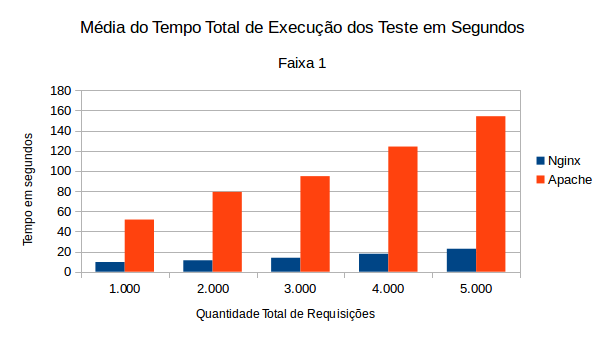
\includegraphics[width=0.6\linewidth]{graficos/grafico1-f1} 
	\caption{Média do Tempo Total de Execução dos Testes - Faixa 1}
	\label{fig:grafico1-f1}
\end{figure}



